%% Grady Wright
%% Boise State University

%% Solutions by Sage Shaw
%% Boise State University

\documentclass[final,oneside,onecolumn]{article}
\usepackage[body={6in,9.5in},top=0.9in,left=1in,dvips]{geometry}
\usepackage{amsmath}
\usepackage{float}
\usepackage{graphicx}
\usepackage{amsfonts}
\usepackage{amssymb}
\usepackage{paralist}
\usepackage{floatflt}
\usepackage{alltt}
\usepackage{color}
%\usepackage{algorithm}
%\usepackage{algorithmic}
\usepackage{url}
\usepackage{subfig}

\definecolor{string}{rgb}{0.7,0.0,0.0}
\definecolor{comment}{rgb}{0.13,0.54,0.13}
\definecolor{keyword}{rgb}{0.0,0.0,1.0}

% Python LstListing
\definecolor{pygreen}{rgb}{0,.4,0}
\definecolor{pyoperator}{rgb}{.8,0,.8}
\definecolor{pycomment}{rgb}{.5,.5,.5}
\definecolor{pyidentifier}{rgb}{0,0,1}
\usepackage{listings}
\usepackage{courier}
\lstset{language=Python,
keywordstyle=\color{pygreen},
stringstyle=\color{string},
commentstyle=\color{pycomment},
%identifierstyle=\color{pyidentifier},
literate=	{+}{{{\color{pyoperator}+}}}{1}
			{*}{{{\color{pyoperator}*}}}{1}
			{-}{{{\color{pyoperator}-}}}{1}
			{/}{{{\color{pyoperator}/}}}{1}
			{**}{{{\color{pyoperator}**}}}{2}
			{@}{{{\color{pyoperator}@}}}{1},
basicstyle=\footnotesize\ttfamily\bfseries
}

\newcommand{\matlab}{\textsc{Matlab\;}}
\newcommand{\matlabs}{\textsc{Matlab}'s\;}
\newcommand{\grads}{[\text{565 only}]}
\newcommand{\ugrads}{[\text{465 only}]}
\newcommand{\maple}{\emph{Maple\;}}
\newcommand{\erf}{\text{erf}}
\newcommand{\sign}{\text{sign}}
\newcommand{\lnorm}{\left\|}
\newcommand{\rnorm}{\right\|}
\newcommand{\ds}{\displaystyle}
\newcommand{\lam}{\lambda}
\newcommand{\ol}{\overline}
\newcommand{\vf}{\mathbf{f}}
\newcommand{\vy}{\mathbf{y}}
\newcommand{\vx}{\mathbf{x}}
\newcommand{\vd}{\mathbf{d}}
\newcommand{\sn}{\text{sn}}
\newcommand{\cn}{\text{cn}}
\newcommand{\dn}{\text{dn}}

\newcommand{\bh}{\hat{b}}
\newcommand{\ah}{\hat{a}}
\newcommand{\xh}{\hat{x}}
\newcommand{\uh}{\hat{u}}
\newcommand{\fh}{\hat{f}}
\newcommand{\bhv}{\hat{\mathbf{b}}}
\newcommand{\ahv}{\hat{\mathbf{a}}}
\newcommand{\xhv}{\hat{\mathbf{x}}}
\newcommand{\uhv}{\hat{\mathbf{u}}}
\newcommand{\fhv}{\hat{\mathbf{f}}}
\newcommand{\uv}{\mathbf{u}}
\newcommand{\vu}{\mathbf{u}}
\newcommand{\vb}{\mathbf{b}}
\newcommand{\fv}{\mathbf{f}}
\newcommand{\ve}{\mathbf{e}}
\newcommand{\vw}{\mathbf{w}}

\usepackage{wasysym}


\newcommand{\fdst}[3]{\left[\begin{array}{ccc} #1 & #2 & #3 \end{array}\right]}

\begin{document}

\renewcommand{\arraystretch}{0.5}

\title{\begin{tabular*}{6.5in}[h]{l@{\extracolsep\fill}cr}
{\bf \large Math 566} & {\bf \large Homework 5} & {\bf \large Sage Shaw} \\
{\bf \large Instructor: Grady Wright} & & {\bf \large Due Nov.\ 9, 2018}\\
\end{tabular*}}
\date{}
\author{}
\maketitle

\thispagestyle{empty}

\begin{enumerate}

\item \emph{Linear multi-step methods} The following are six suggestions for linear multistep methods for solving
the initial value problem $y'=f(t,y(t))$, $a \leq t \leq b$, $y(a) = y_0$:
\begin{enumerate}
   \item $y^{n+1} = \frac{1}{2}\left[y^{n} + y^{n-1}\right] + 2kf^{n}$
   \item $y^{n+1} = y^n$
   \item $y^{n+1} = y^{n-3} + \frac{4}{3}k\left[f^{n} + f^{n-1} + f^{n-2}\right]$
   \item $y^{n+1} = y^{n-1} + \frac{1}{3}k\left[7f^{n} - 2f^{n-1} + f^{n-2}\right]$
   \item $y^{n+1} = \frac{8}{19}\left[y^{n} - y^{n-2}\right] + y^{n-3} + \frac{6}{19}k\left[f^{n+1} + 4f^{n} + 4f^{n-2} + f^{n-3}\right]$
   \item $y^{n+1} = -y^{n} + y^{n-1} + y^{n-2} + 2h\left[f^{n} + f^{n-1}\right]$
\end{enumerate}
Here $k$ is the time-step, i.e.\ $k=(b-a)/N$ for some positive integer $N$.

The (incomplete) table below summarizes their properties.  Complete the missing
entries of this table (you need not supply any derivations), draw the corresponding
stencil, state the generating polynomials $\rho(w)$ and $\sigma(w)$, and state
the number of steps $r$.
\begin{center}
\begin{tabular}{|c|l|l|c|c|c|l|c|}
\hline
case & char. eq & roots & stab-   & accu- & consis- & leading & conver- \\
     &          &       & ility & racy  & tency   & error term & gence \\
\hline
(a)  & $w^2 - \frac{1}{2}w - \frac{1}{2}=0$ & $1,-\frac{1}{2}$ & Yes & 
0 &  & $-\frac{1}{2}k f'(\xi)$ & \\
& & & & & & & \\
(b)  &  & & & 0 & No  & & No \\
& & & & & & & \\
(c)  &  &  &  &   & Yes  &  & Yes \\
& & & & & & & \\
(d)  &  &  &  & 3 &      & $\frac{1}{3}k^4 f^{(4)}(\xi)$ & Yes \\
& & & & & & & \\
(e)  & $w^4 - \frac{8}{19}w^3 + \frac{8}{19}w-1=0$ & $\pm 1,\frac{4}{19}\pm \frac{\sqrt{345}}{19}i$ &  & 
6 &  & $-\frac{6}{665}k^7 f^{(7)}(\xi)$ & \\
& & & & & & & \\
(f)  &  &  &  & 2 & Yes & $\frac{2}{3}k^3 f^{(3)}(\xi)$ & \\
& & & & & & & \\
\hline
\end{tabular}
\end{center}
\bigbreak

%%%%%%%%%%%%%%%%%%%%%
{\large \bf Solution}: Here is the completed table.
\begin{center}
	\begin{tabular}{|c|l|l|c|c|c|l|c|}
		\hline
		case & char. eq & roots & stab-   & accu- & consis- & leading & conver- \\
		&          &       & ility & racy  & tency   & error term & gence \\
		\hline
		(a)  & $w^2 - \frac{1}{2}w - \frac{1}{2}=0$ & $1,-\frac{1}{2}$ & Yes & 
		0 &\textbf{No}  & $-\frac{1}{2}k f'(\xi)$ &\textbf{No} \\
		& & & & & & & \\
		(b)  &$\boldsymbol{\omega-1=0}$  &$\mathbf{1}$ &\textbf{Yes} & 0 & No  &$\boldsymbol{f(\xi)}$ & No \\
		& & & & & & & \\
		(c)  &$\boldsymbol{\omega^4-1=0}$  &$\mathbf{\pm 1, \pm i}$  &\textbf{Yes}  & \textbf{2} & Yes  & $\boldsymbol{\frac{4}{3}k^3 f^{(3)}(\xi)}$ & Yes \\
		& & & & & & & \\
		(d)  &$\boldsymbol{\omega^3-\omega=0}$  &$\mathbf{0, \pm 1}$  &\textbf{Yes}  & 3 & \textbf{Yes}    & $\frac{1}{3}k^4 f^{(4)}(\xi)$ & Yes \\
		& & & & & & & \\
		(e)  & $w^4 - \frac{8}{19}w^3 + \frac{8}{19}w-1=0$ & $\pm 1,\frac{4}{19}\pm \frac{\sqrt{345}}{19}i$ &\textbf{Yes}  & 
		6 & \textbf{Yes}  & $-\frac{6}{665}k^7 f^{(7)}(\xi)$ & \textbf{Yes} \\
		& & & & & & & \\
		(f)  &$\boldsymbol{\omega^3+\omega^2-\omega-1=0}$  &$\mathbf{\pm 1}$  &\textbf{No}  & 2 & Yes & $\frac{2}{3}k^3 f^{(3)}(\xi)$ & \textbf{No} \\
		& & & & & & & \\
		\hline
	\end{tabular}
\end{center}

\bigbreak
	%%%%%%%%%%%%%%%%%%%%%%%%%
	(a) Two step method \\
	$\rho(\omega) = \omega^2 - \frac{1}{2}\omega - \frac{1}{2}$ \\
	$\sigma(\omega) = 2 \omega$ \\
	\begin{tabular}{c|cc}
		$r_{n+1}$ & $\square$ & \\ \hline
		$r_{n}$ & $\blacksquare$ & $\CIRCLE$\\
		$r_{n-1}$ & $\blacksquare$ & \\
	\end{tabular}
\bigbreak
	%%%%%%%%%%%%%%%%%%%%%%%%%
	(b)  One step method \\
	$\rho(\omega) = \omega - 1$ \\
	$\sigma(\omega) = 0$\\
	\begin{tabular}{c|cc}
		$r_{n+1}$ & $\square$ & \\ \hline
		$r_{n}$ & $\blacksquare$ & \\
	\end{tabular}
\bigbreak
	%%%%%%%%%%%%%%%%%%%%%%%%%
	(c) Four step method \\
	$\rho(\omega) = \omega^4 - 1$ \\
	$\sigma(\omega) = \frac{4}{3} ( \omega^3 + \omega^2 + \omega )$\\
	\begin{tabular}{c|cc}
		$r_{n+1}$ & $\square$ &  \\ \hline
		$r_{n}$   & & $\CIRCLE$\\
		$r_{n-1}$ & & $\CIRCLE$\\
		$r_{n-2}$ & & $\CIRCLE$\\
		$r_{n-3}$ & $\blacksquare$ & \\
	\end{tabular}
\bigbreak
	%%%%%%%%%%%%%%%%%%%%%%%%%
	(d) Three step method \\
	$\rho(\omega) = \omega^3 - \omega$ \\
	$\sigma(\omega) = \frac{1}{3} ( 7\omega^2 -2 \omega + \omega )$\\
	\begin{tabular}{c|cc}
		$r_{n+1}$ & $\square$ &  \\ \hline
		$r_{n}$   & & $\CIRCLE$\\
		$r_{n-1}$ & $\blacksquare$ & $\CIRCLE$\\
		$r_{n-2}$ & & $\CIRCLE$ \\
	\end{tabular}
\bigbreak
	%%%%%%%%%%%%%%%%%%%%%%%%%
	{(e) Four step method \\
	$\rho(\omega) = \omega^4 - \frac{8}{19}\omega^3 + \frac{8}{19}\omega - 1$\\
	$\sigma(\omega) = \frac{6}{19} ( \omega^4 +4\omega^3 + 4\omega + 1)$\\
	\begin{tabular}{c|cc}
		$r_{n+1}$ & $\square$ & $\Circle$ \\ \hline
		$r_{n}$   & $\blacksquare$ & $\CIRCLE$\\
		$r_{n-1}$ &  & \\
		$r_{n-2}$ & $\blacksquare$ & $\CIRCLE$ \\
		$r_{n-3}$ & $\blacksquare$ & $\CIRCLE$ \\
	\end{tabular}}
\bigbreak
	%%%%%%%%%%%%%%%%%%%%%%%%%
	{(f) Three step method \\
	$\rho(\omega) = \omega^3 + \omega^2 - \omega - 1$\\
	$\sigma(\omega) = 2 ( \omega^2 + \omega)$\\
	\begin{tabular}{c|cc}
		$r_{n+1}$ & $\square$ & \\ \hline
		$r_{n}$   & $\blacksquare$ & $\CIRCLE$\\
		$r_{n-1}$ & $\blacksquare$ & $\CIRCLE$\\
		$r_{n-2}$ & $\blacksquare$ &  \\
	\end{tabular}}
		

\bigbreak
%%%%%%%%%%%%%%%%%%%%%%%%%%%%%%%%%%%%%%%%%%%%%%%%%%%%%%%%%%%%%%%%%%%%%%%%%%%%%%%%%%%%%%%%%%%%%%%%%%%%%%%
\item \emph{Predictor-Corrector method}
\begin{enumerate}
\item Implement a function in the language of your choosing for numerically solving the general \emph{vector-valued} IVP 
\begin{eqnarray*}
 \vy' = \vf(t,\vy), & a \leq t \leq b, & \vy(a) = \vy_0\;\; 
 (\vy\in\mathbb{R}^n),
\end{eqnarray*}
using the \emph{fourth-order}, predictor-corrector method of AB4 (4-step method) and AM4 (3-step method):
\begin{eqnarray*}
   \vy^{*} & = & \vy^{n} + \frac{k}{24}[55\vf(t_{n},\vy^n) - 59\vf(t_{n-1},\vy^{n-1})
    + 37\vf(t_{n-2},\vy^{n-2}) - 9\vf(t_{n-3},\vy^{n-3})]\;\; (\text{AB4 predictor}) \\
   \vy^{n+1}     & = & \vy^{n} + \frac{k}{24}[9\vf(t_{n+1},\vy^{*}) 
    + 19\vf(t_{n},\vy^{n}) - 5\vf(t_{n-1},\vy^{n-1})
    + \vf(t_{n-2},\vy^{n-2})]\;\; (\text{AM4 corrector})\; \\
    & & j=3,4,\ldots,N-1\;.
\end{eqnarray*}
Your function should be called \verb|abm4|, and take as input a function that
represents the vector-valued function $\vf(t,\vy)$, $a$, $b$, the initial
condition $\vy_0$, and the number of steps to take $N$.  The output of your
function should be a vector \verb|t| containing all of the time-steps,
and a matrix \verb|y| containing the numerical solution of all the components of
the system $\vy$ at each time-step. 

You will need to obtain the three values $\vy_1$, $\vy_2$, and $\vy_3$ to get your \verb|abm4| function started.  These values should be obtained with a fourth-order accurate method to keep the scheme consistent.  The easiest approach is to use the standard fourth-order Runge-Kutta method (see Example 5.13 on p.\ 126 of the book).

Turn in a printed listing and e-mail me your program(s).

\begin{quote}
   \underline{\bf{Note:}} Your function must be entirely general.  This means that I
   should be able to create my own function for any $f(t,\vy)$, the
   values $a$, $b$, and $\vy_0$, and use your program \verb|abm4| to try
   and solve the problem.  Furthermore, your program should minimize the number
   of times the function $f(t,\vy)$ needs to be called.
\end{quote}

\bigbreak
%%%%%%%%%%%%%%%%%%%%%
{\large \bf Solution}:

\begin{lstlisting}[language=Python]
def rk4(f, a, b, y0, N):
	if np.ndim(y0) is 0:
		ys = np.zeros(N+1)
	else:
		ys = np.zeros((N+1,len(y0)))
	
	k = (b - a)/N
	ys[0] = y0
	ts = np.linspace(a,b,N+1)
	
	for i in range(N):
		t = ts[i]
		y1 = ys[i]
		f1 = f(t,y1)
		y2 = y1 + k/2*f1
		f2 = f(t+k/2, y2)
		y3 = y1 + k/2*f2
		f3 = f(t+k/2, y3)
		y4 = y1 + k*f3
		ys[i+1] = y1 + k/6*( f1 + 2*f2 + 2*f3 + f(t+k, y4) )
	
	return ts, ys

def abm4(f, a, b, y0, N):
	if np.ndim(y0) is 0:
		ys = np.zeros(N+1)
	else:
		ys = np.zeros((N+1,len(y0)))

	k = (b - a)/N
	ys[0] = y0
	ts = np.linspace(a,b,N+1)
	
	temp, ys[:4] = rk4(f, a, a+3*k, y0, 3)
	fs = np.zeros(ys.shape)
	fs[0] = f(ts[0], ys[0])
	fs[1] = f(ts[1], ys[1])
	fs[2] = f(ts[2], ys[2])
	
	for i in range(3, N):
		fs[i] = f(ts[i], ys[i])
		y_star = ys[i] + k/24*( 55*fs[i] - 59*fs[i-1] + 37*fs[i-2] - 9*fs[i-3] )
		ys[i+1] = ys[i] + k/24*( 9*f(ts[i+1],y_star) + 19*fs[i] - 5*fs[i-1] + fs[i-2] )
	
	return ts, ys
\end{lstlisting}

%%%%%%%%%%%%%%%%%%%%%%%%%%%%%%%%%%%%%%%%%%%%%%%%%%%%%%%%%%%%%%%%%%%%%%%%%%%%%%%%%%%%%%%%%%%%%%%%%%%%%%%
\item Consider the initial value problem
\begin{eqnarray*}
    y' = 1 + \frac{y}{t} + \left(\frac{y}{t}\right)^2, & 
    1 \leq t \leq 3, & y(1) = 0\;,
\end{eqnarray*}
where the exact solution is $y(t)=t\tan(\log(t))$.  Use your abm4 method from 
part (a) to numerically solve this IVP for $1 \leq t \leq 3$ for the different $N$ values 
[50,100,200,400].  Compute the error in the numerical solution at $t=3$ and make either a 
table or a graph clearly showing fourth-order convergence of the solution. On a single graph, 
plot the solution for $N=100$ over the interval  $1 \leq t \leq 3$.

\bigbreak
%%%%%%%%%%%%%%%%%%%%%
{\large \bf Solution}: The code above was used to test values of $N=[50,100,200,400,800, 1600, 3200, 6400]$. The extra values are necessary to realize 4th order convergence. The results shown below indicate 4th order convergence.
\begin{figure}[H]
	\centering
	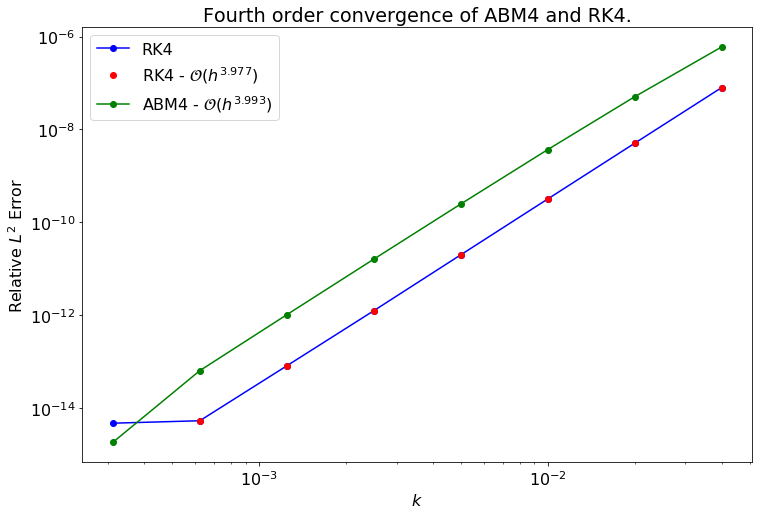
\includegraphics[width=.8\linewidth]{hw5_2b_convergence}
	%\captionof{figure}{A figure}
\end{figure}

\begin{figure}[H]
	\centering
	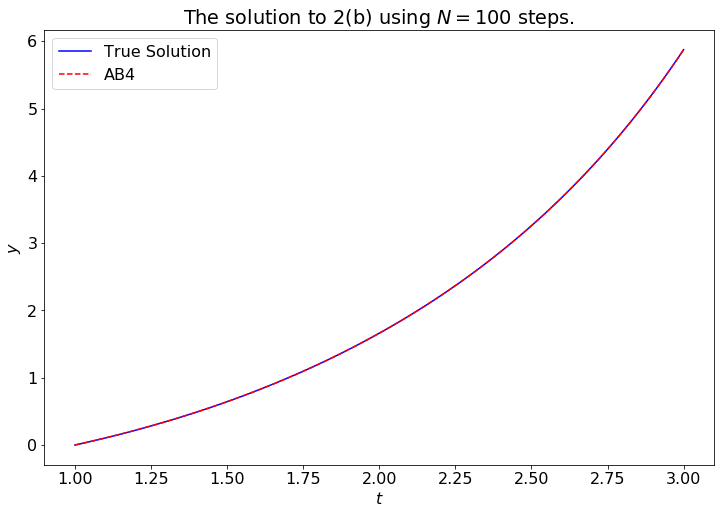
\includegraphics[width=.8\linewidth]{hw5_2b_plot}
	%\captionof{figure}{A figure}
\end{figure}

\end{enumerate}

\bigbreak
%%%%%%%%%%%%%%%%%%%%%%%%%%%%%%%%%%%%%%%%%%%%%%%%%%%%%%%%%%%%%%%%%%%%%%%%%%%%%%%%%%%%%%%%%%%%%%%%%%%%%%%
\item \emph{Satellite oribts} The initial value problem (IVP) below simulates the trajectory of a 
small satellite in the Earth-moon system, where all orbits lie in a plane:
\begin{equation*}
\begin{array}{rll}
x_1''(t) = x_1(t) + 2x_2'(t) - \mu^{*}\dfrac{x_1 + \mu}{D_1} - \mu\dfrac{x_1 - \mu^{*}}{D_2}, & x_1(0) = 0.994,\;x_1'(0) = 0,\\
\\
x_2''(t) = x_2(t) - 2x_1'(t) - \mu^{*}\dfrac{x_2}{D_1} - \mu\dfrac{x_2}{D_2}, & x_2(0) = 0,\;x_2'(0) = -2.0015851063790825,\\
\end{array}
\end{equation*}
where,
\begin{equation*}
\begin{array}{c}
0 \leq t \leq b=17.06521656015796, \\
\mu = 0.012277471,\;\; \mu^{*} = 1-\mu, \\
D_1 = ((x_1 + \mu)^2 + x_2^2)^{3/2}, \;\; D_2 = ((x_1 - \mu^{*})^2 + x_2^2)^{3/2}, \\
\end{array}
\end{equation*}
The mass of the satellite is neglected.  The coordinate system moves so that the
origin is the center of mass of the Earth and moon, and it rotates so that the
Earth and moon lie on the $x_1$ axis a distance 1 apart (the Earth is just left of
the origin, and the moon is just left of (1,0)). The constants are chosen so that
$\vx(b) = \vx(0)$.
\begin{enumerate}
   \item Use your \verb|abm4| function (with the RK4 modification) to compute one
   period of the orbit with 3000 time-steps.  Produce a phase portrait of $x_2$ vs.
   $x_1$. 
\bigbreak
%%%%%%%%%%%%%%%%%%%%%
{\large \bf Solution}: Our first step is to pose this problem as a system of first order ODEs. We make the following substitutions
\begin{align*}
	y_0 &= x_1 \\
	y_1 &= x'_1 = y_0' \\
	y_2 &= x_2 \\
	y_3 &= x'_2 = y_2'
\end{align*}
which leads to the first order system of ODES
\begin{equation*}
	\begin{array}{rll}
	y_0' &= y_1, & y_0(0) = 0.994, \\
	y_1' &= y_0 + 2y_3 - \mu^{*}\dfrac{y_0 + \mu}{D_1} - \mu\dfrac{y_0 - \mu^{*}}{D_2}, & y_1(0) = 0,\\
	y_2' &= y_3, & y_2(0) = 0, \\
	y_3' &= y_2 - 2y_1 - \mu^{*}\dfrac{y_2}{D_1} - \mu\dfrac{y_2}{D_2}, & y_3(0) = -2.0015851063790825
	\end{array}
\end{equation*}
where,
\begin{equation*}
	\begin{array}{c}
	0 \leq t \leq b=17.06521656015796, \\
	\mu = 0.012277471,\;\; \mu^{*} = 1-\mu, \\
	D_1 = ((y_0 + \mu)^2 + y_2^2)^{3/2}, \;\; D_2 = ((y_0 - \mu^{*})^2 + y_2^2)^{3/2}. \\
	\end{array}
\end{equation*}
We can now apply our ABM4 function to this system. The plot below comes from using ABM4 with $N=3000$ time steps. RK4 is also shown for comparison.
   
\begin{figure}[H]
	\centering
	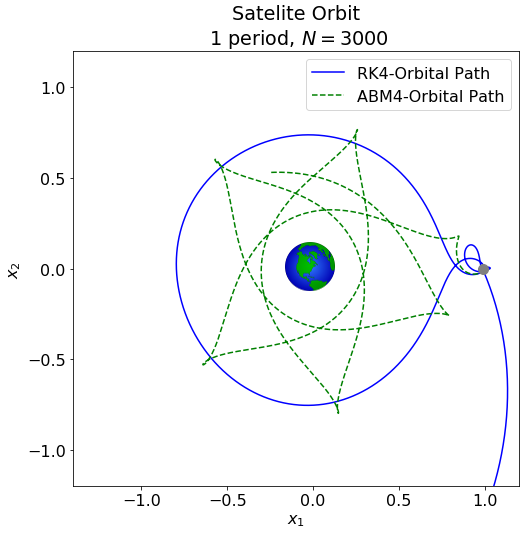
\includegraphics[width=.6\linewidth]{hw5_3a_3ksteps}
	%\captionof{figure}{A figure}
\end{figure}

This path does not seem realistic and does not seem periodic. When we increase the time steps to $N=18,000$ we get something much more appropriate.
\begin{figure}[H]
	\centering
	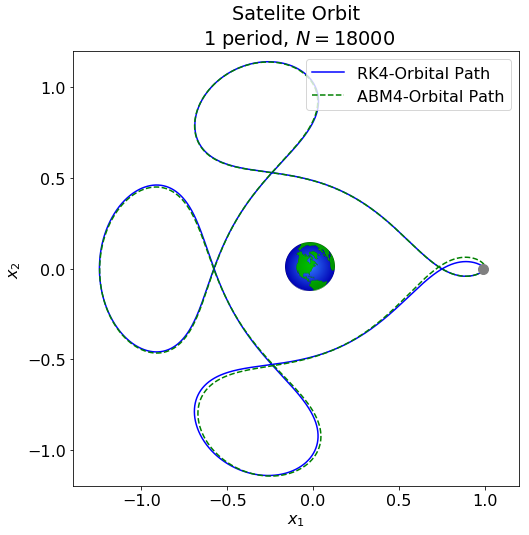
\includegraphics[width=.6\linewidth]{hw5_3a_18ksteps}
	%\captionof{figure}{A figure}
\end{figure}

\bigbreak
%%%%%%%%%%%%%%%%%%%%%%%%%%%%%%%%%%%%%%%%%%%%%%%%%%%%%%%%%%%%%%%%%%%%%%%%%%%%%%%%%%%%%%%%%%%%%%%%%%%%%%%
   \item Repeat part (a), but now compute the orbit for 3 periods using 9000 time-steps.
   Explain what is wrong with the results.  Is it possible to make the problem go away by increasing the number of time-steps? Explain.

\bigbreak
%%%%%%%%%%%%%%%%%%%%%
{\large \bf Solution}: Here we plot the solution over three periods with $N=9,000$.
\begin{figure}[H]
	\centering
	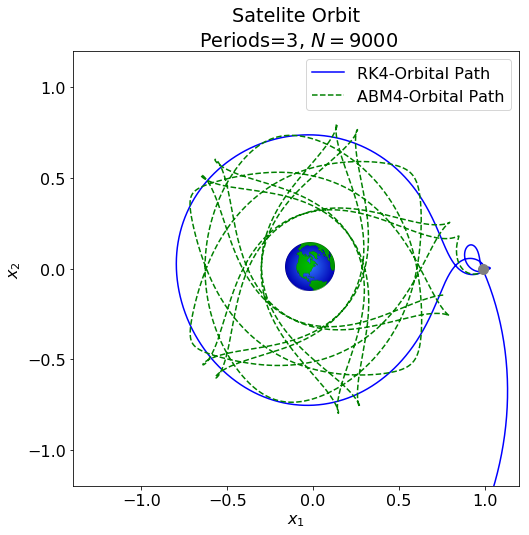
\includegraphics[width=.6\linewidth]{hw5_3a_3periods_9ksteps}
	%\captionof{figure}{A figure}
\end{figure}
As before, the step-size is not refined enough to generate a realistic solution. At $N=27,000$ we have a more realistic trajectory.
\begin{figure}[H]
	\centering
	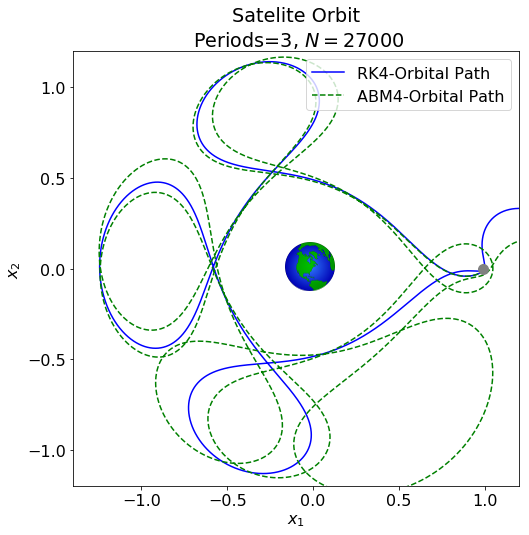
\includegraphics[width=.6\linewidth]{hw5_3a_3periods_27ksteps}
	%\captionof{figure}{A figure}
\end{figure}
Though the true solution is periodic, an increased step-size does not give periodic solutions. The issue is that the forcing function is not Lipschitz over the entire domain. In particular the terms $\frac{1}{D_1}$ and $\frac{1}{D_2}$ are singular (in the $x_1, x_2$ domain) at the points $(-\mu, 0)$ and $(\mu^*,0)$ respectively. As the satellite approaches either of these points the growth in the derivatives is unbounded. 
\bigbreak

Practically speaking, if we simply exclude these points from our domain the problem will be Lipschitz, but we will need to assume that the trajectory does not pass through either of the singularities. In practice, though some sufficiently restricted domain may fix this, the Lipschitz constant will be very large since our starting value is so close to $(\mu^*,0)$. If we look at a satellite, call it Satellite-2, with a different starting position: $(1.2, 0)$. and the same initial velocity, we get a path (that may not be periodic in this changing reference frame) that does not pass near to the two singularities. Below is the solution to the trajectory of Satellite-2 using ABM4 and RK4 for $N=500, 3000$ over the same time interval (not technically a period anymore). Notice that both methods are indistinguishable by the eye for both values of $N$. This agrees with the hypothesis that passing near the singularities leads to ill-posedness of the problem.
\begin{figure}[H]
	\centering
	\subfloat[$N=500$]{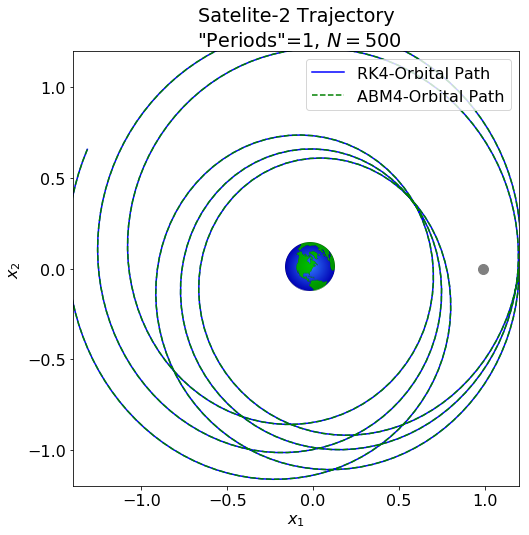
\includegraphics[width=.5\linewidth]{hw5_3b_500steps}}
	\subfloat[$N=3000$]{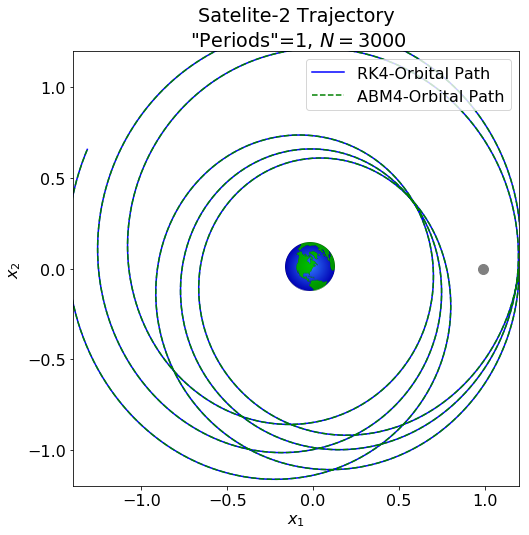
\includegraphics[width=.5\linewidth]{hw5_3b_3ksteps}}
\end{figure}

   
\end{enumerate}

\bigbreak
%%%%%%%%%%%%%%%%%%%%%%%%%%%%%%%%%%%%%%%%%%%%%%%%%%%%%%%%%%%%%%%%%%%%%%%%%%%%%%%%%%%%%%%%%%%%%%%%%%%%%%%
\item \emph{Derivation of linear multistep methods} Consider the following third-order accurate LMM
\begin{equation*}
y^{n+1} = y^{n-1} + \dfrac{k}{3}\left[7f^{n} - 2f^{n-1} + f^{n-2}\right]\;,
\end{equation*}
\begin{enumerate}
\item Derive this method using any technique you desire.
\begin{quote}
{\footnotesize \underline{Hint:} The most straightforward approach is to
consider the appropriate approximation to the formal solution
\begin{equation*}
   y(t^{n+1}) = y(t^{n-1}) + \int_{t^{n-1}}^{t^{n+1}} f(t,y(t) dt
\end{equation*}
of the general IVP $y'(t) = f(t,y)$.
}\end{quote}

\bigbreak
%%%%%%%%%%%%%%%%%%%%%
{\large \bf Solution}: As discussed in class the coefficients $\beta_r$ can be derived by interpolating the points $(0, f^{n-2}), (1, f^{n-1}), (2, f^{n})$ (centered at $t_{n-2}$ and scaled by $\frac{1}{k}$) with a polynomial, and then approximating the integral of this polynomial. The following \texttt{Sympy} code constructs the Lagrange interpolating polynomial $L_j(t)$, and then integrates to find the coefficient on $kf^{n-j}$.
\begin{lstlisting}[language=Python]
from sympy import *
init_printing() # Renders output as LaTeX
t = symbols('t')
for j in range(2, -1, -1):
	L = 1 # Construct L_j in a loop
	for i in range(3):
		if i != j:
			L *= (t-i)/(j-i)
	I = integrate(L, (t, 1, 3))
	display(I)
\end{lstlisting}
The output it gives is $\frac{7}{3}, -\frac{2}{3}, \frac{1}{3}$ corresponding to $f^n, f^{n-1}$ and $f^{n-2}$ respectively. Rescaling by $k$ and centering at $t_{n-2}$ we have the desired result.
\begin{equation*}
y^{n+1} = y^{n-1} + \dfrac{k}{3}\left[7f^{n} - 2f^{n-1} + f^{n-2}\right]\;,
\end{equation*}

\bigbreak
%%%%%%%%%%%%%%%%%%%%%%%%%%%%%%%%%%%%%%%%%%%%%%%%%%%%%%%%%%%%%%%%%%%%%%%%%%%%%%%%%%%%%%%%%%%%%%%%%%%%%%%
\item Plot the stability domain for this LMM and include on your plot the stability
domain for the third order Adams-Bashforth method (AB3).  Compare and contrast the
two stability domains in terms of the problems they might be good for solving.
\end{enumerate}

\bigbreak
%%%%%%%%%%%%%%%%%%%%%
{\large \bf Solution}: This LMM is stable if all of the roots of the characteristic equation $\rho(\omega) - \xi \sigma(\omega)$ have magnitude less than than or equal to one, with no more than one root of magnitude equal to one. Here $\xi = \lambda k$ where $k$ is the step-size and $\lambda$ is the largest (in magnitude) eigenvalue of the system of differential equations. If we set the characteristic equation equal to zero, and solve for $\xi$ as a function of $\omega$ we have $\xi(\omega) = \frac{\rho(\omega)}{\sigma(\omega)}$. For any given value of $\omega$ this function yields the value of $\xi$ such that the characteristic equation $\rho(\omega) - \xi \sigma(\omega)$ has a root of $\omega$. If we map the complex unit circle $\{\omega = e^{i\theta} \mid \theta \in [0, 2\pi)\}$ through our function $\xi(\omega)$ we have a curve that shows all values of $xi$ such that the characteristic equation has a root with magnitude one.
\bigbreak

This curve may self-intersect, but will certainly be closed and must partition the complex plane. All values of $xi$ in a given partition will lead to stability in the method if any point in that partition leads to stability in the algorithm. Testing one point in each partition is sufficient. 
\bigbreak

The plot below shows the region of absolute stability for both the LMM given above, and Adams Bashforth  3. ABM3 is stable in the shaded region where this LMM seems to be nowhere stable. 

\begin{figure}[H]
	\centering
	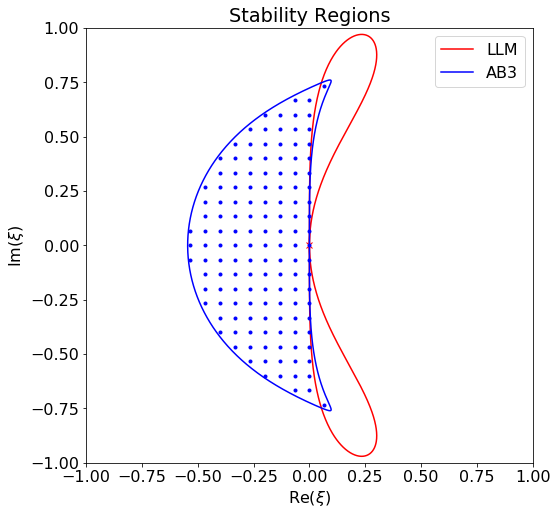
\includegraphics[width=.6\linewidth]{hw5_p4_stability}
	%\captionof{figure}{A figure}
\end{figure}

This is an unexpected result, and expect it is incorrect. When tested using the model problem $y' = y$, $y_0 = 1$ it gives 3rd order convergence as seen the plot below. This seems to contradict that the positive real axis is not in the stability domain. 

\begin{figure}[H]
	\centering
	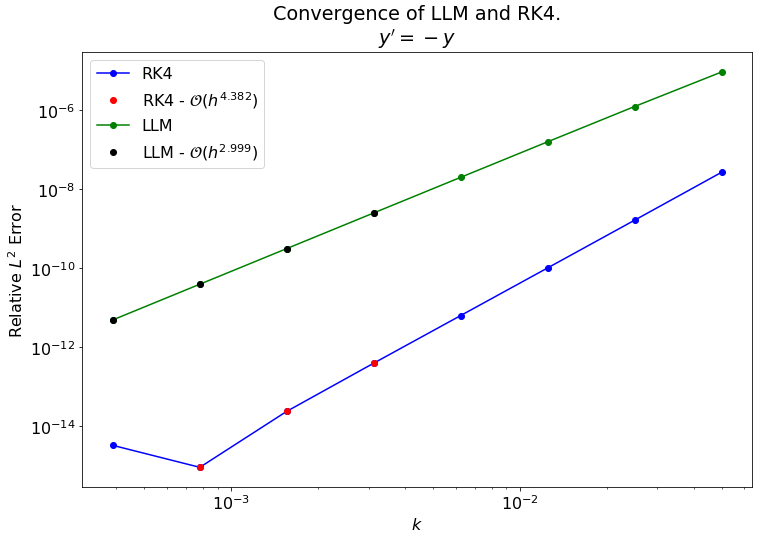
\includegraphics[width=.9\linewidth]{hw5_p4b_stable_order}
	%\captionof{figure}{A figure}
\end{figure}

However, when applied to the problem $y'' = 16 y' - 68; y(0)=0; y'(0)=8$, which has eigenvalues of $\lambda = 2 \pm 8i$, there are values of $k$ that put $\xi = \lambda k$ in the interior of the "boomerang" shape. The plot below shows that when $k = 1, \frac{1}{2}, \frac{1}{4}, \frac{1}{8}$ that the LMM is unstable. 

\begin{figure}[H]
	\centering
	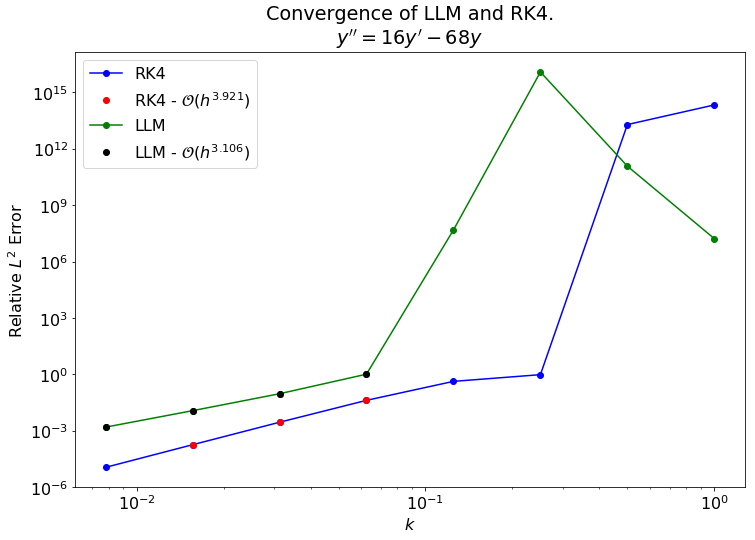
\includegraphics[width=.9\linewidth]{hw5_p4b_unstable_order}
	%\captionof{figure}{A figure}
\end{figure}

Thus it would seem that the true stability region is as shown in the plot below. If this is the true stability region then this LMM could be used almost any time that AB3 could be used. The only case in which one would prefer to use AB3 over this LMM is when the system of ODEs has an eigenvalue that has a positive real component, but also has an imaginary component that is much larger (in magintude), such as $\lambda = 2+800i$. In practice both will be unstable for some small time step, but there will be a region of small time steps where AB3 is stable but this LMM is unstable.

\begin{figure}[H]
	\centering
	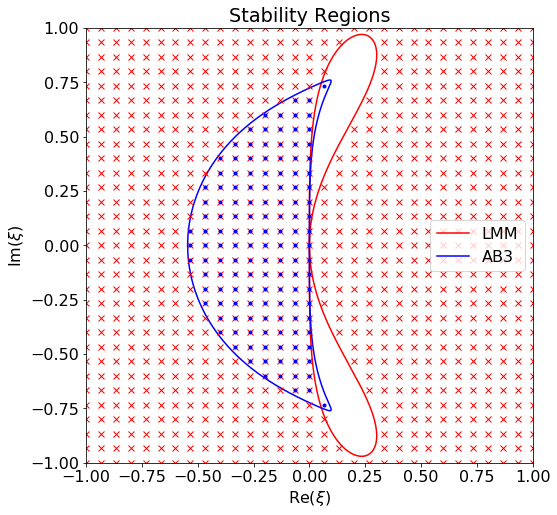
\includegraphics[width=.6\linewidth]{hw5_p4b_true_region}
	%\captionof{figure}{A figure}
\end{figure}

In general, AB3 is good for solving problems that have non-positive real eigenvalues. This LLM is good for solving all problems except those that have eigenvalues with positive real component much smaller than the magnitude of the imaginary component. 

\end{enumerate}
\bibliography{../Ref}
\bibliographystyle{unsrt}


\end{document}
